\label{introducao}

A resolução de diversos problemas se dá na forma de algoritmos, de instruções bem definidas. No entanto, alguns algoritmos podem pedir inúmeras instruções até concluírem, o que pode até mesmo inviabilizar a solução encontrada. A Inteligência Artificial pode atuar sobre tais problemas de modo a interagir com o problema e aprender com ele a encontrar uma solução. Ótimos candidatos a esta tarefa são os chamados \emph{algoritmos evolutivos (AE)}.

Algoritmos evolutivos são aqueles que se baseiam nos princípios de evolução natural da Biologia, e são aplicados em um modo particular de solução de problemas: o da tentativa-e-erro. Tais algoritmos possuem um framework atuante sobre diferentes \emph{gerações} de um problema, por meio da alteração ou manutenção dos seres existentes na \emph{população} \cite{eiben2003introduction}. A população, em termos computacionais, pode ser vista como o conjunto de parâmetros de interesse retornados pelo problema, enquanto uma geração seria a população resultante de um ciclo de iterações do AE sobre o problema. Tal framework pode ser visto na figura \ref{fig:evolution-framework}.

\begin{figure}[ht!]
    \centering	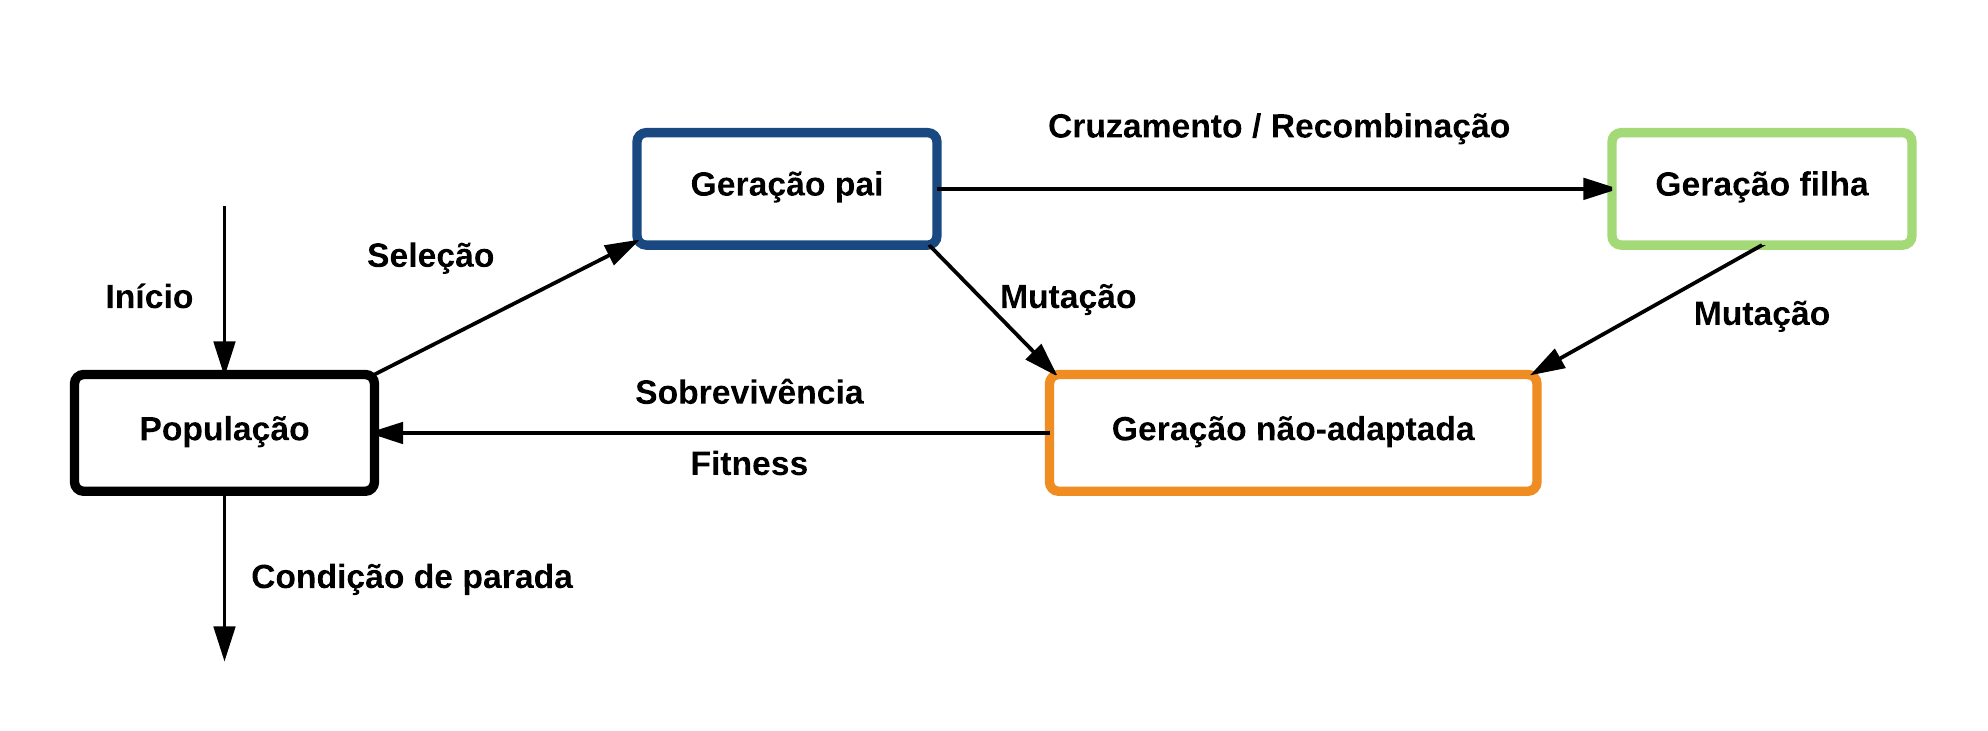
\includegraphics[width=1.0\textwidth]{evolution-framework.png}
    \caption{Framework de um algoritmo evolutivo.}
    \label{fig:evolution-framework}
\end{figure}

Similar ao processo evolutivo, seus componentes principais são as operações de variação (mutação e recombinação) e de seleção (seleção da geração pai e sobrevivência da geração filha), chamados aqui simplesmente de \emph{operações de evolução} \cite{eiben2011parameter}. É possível ver a \emph{mutação} como a atribuição de um (novo) valor aleatório. A \emph{recombinação} atribuiria o valor médio de uma amostra da população. \emph{Seleção} envolve uma escolha a dedo dos melhores exemplares, e \emph{sobrevivência} envolve a rejeição de um exemplar que não seja tão bom.

Em termos de implementação, o AE deve ser tal que, uma vez aplicado sobre uma população, o desenvolvimento sequencial de gerações é feito automaticamente. Para isso, é necessário passar por quatro etapas \cite{eiben2011parameter}:

\begin{enumerate}[label={[\arabic*]}]
	\item Implementação do AE e de suas operações de evolução;
	\item Implementação de problemas compatíveis com a aplicação do AE;
	\item Otimização do AE quando aplicado a um problema;
	\item Definição e utilização da função utilidade do AE. 
\end{enumerate}

Para [1], pensando que mais de um problema se utilizará do AE, e que cada problema terá populações de complexidades diferentes. É necessário implementar operações de evolução diferentes para cada tipo de população, mas que obedeçam sempre à mesma sequência de execução.

Para [2], é necessário não só deixar a população de um problema acessível ao AE, mas também dizer ao problema quão próxima de uma solução uma geração se encontra, ou quão melhor é uma geração frente às demais. Tal escala é trazida por uma função de \emph{fitness}. Por exemplo, se um problema envolver o encontro das raízes de um polinômio, uma boa função de fitness para um indivíduo $x_k$ da população poderia ser definida por $|f(x_k)|$, indicando uma melhor solução se o valor obtido for menor ou próximo de 0.

Para [3], é possível associar a expressividade das diferentes operações de evolução a valores numéricos (normalmente indo de 0 - sem expressão - a 1 - expressividade máxima). Tais parâmetros, chamados de \emph{parâmetros de evolução}, são comumente representados por vetores e ditam como o AE agirá sobre um problema. Um bom ajuste destes parâmetros é fundamental para o encontro de boas soluções e uma convergência rápida do algoritmo \cite{eiben1999parameter}.

No entanto, obter um bom vetor de parâmetros não é uma tarefa simples, e simplesmente “chutar” valores já foi comprovado ser algo ineficiente \cite{smit2009comparing}. Tal tarefa é comumente deixada para os algoritmos de ajuste ou de \emph{tuning}, os quais são executados sobre o AE antes de se analisar a aplicação do mesmo sobre o problema. A etapa [3] se mostra análoga à etapa de treinamento de um algoritmo de aprendizado.

Para [4], após ajustar o vetor de parâmetros de um AE, é necessário não só aplicá-lo ao problema, mas também é necessário verificar a qualidade das soluções obtidas ao longo das gerações. Isso é feito por meio da \emph{função utilidade}, a qual determina valores ou métricas de análise das soluções obtidas para um problema. Como é necessário analisar as respostas obtidas, os parâmetros podem se utilizar da função de fitness do problema. 

Como a essência do AE é a tentativa-e-erro, tais métricas advêm de métodos estatísticos, como médias, medianas e desvios padrões, e seus valores são calculados sobre diversas execuções completas do AE sobre um problema. Não é possível, no entanto, atribuir significado a cada uma das métricas, o que pede a obtenção de várias delas em busca de uma análise coerente. Não só isso, se pensarmos em performance, a velocidade de convergência para boas soluções também precisa ser medida \cite{eiben2011parameter}.

Com as quatro etapas concluídas, aplica-se o AE ao problema de interesse, e os resultados são analisados de acordo com os valores trazidos pela função utilidade.

\section{Motivação}

É difícil por si só garantir que um algoritmo evolutivo encontre boas soluções para os problemas mais simples, dada a natureza de sua implementação. Garantir uma execução eficiente do mesmo é fundamental.

\section{Objetivo}

Este trabalho propôs implementar um algoritmo evolutivo que siga as quatro etapas apresentadas acima, de tal forma que ele seja capaz de atuar sobre problemas determinados e encontrar boas soluções com poucas gerações.

\section{Abordagem}

A proposta foi complexa, pois as quatro etapas de criação do algoritmo são interdependentes. A etapa mais crítica foi a [1], que definiu o AE e o esqueleto de implementação de todas as outras etapas. As etapas [2] e [3] precisaram ter seus problemas/algoritmos bem definidos desde o início, para não atrapalharem o desenvolvimento em estágios avançados do trabalho. A etapa [4] precisou implementar diversas métricas ao longo de seu desenvolvimento, de modo a trazer as análises mais abrangentes possíveis para os problemas.

Para a etapa [2], foram escolhidos os seguintes problemas:

\begin{itemize}

	\item \textbf{Problema Onemax \cite{giguere1998population}:} dado um conjunto de 100 bits iniciados em 0, o AE deve ser capaz de tornar todos os bits iguais a 1. A função de fitness avalia quantos bits estão iguais a 1 ao final de uma geração (quando maior o valor, melhor, sendo 100 a solução ótima);

	\item \textbf{O problema das 8 rainhas \cite{campbell1977gauss}:} posicionando oito rainhas inicialmente em posições aleatórias sobre um tabuleiro de xadrez 8x8, o AE deve ser capaz de reposicioná-las de tal forma que uma rainha não seja capaz de atacar as demais. A função de fitness avalia quantas rainhas podem se atacar em uma dada geração (quanto mais próximo de zero, melhor).

\end{itemize}

Para a etapa [3], optou-se por escolher um algoritmo de tuning vastamente utilizado e comparado com outros em termos de performance para múltiplas literaturas \cite{eiben2011parameter, smit2009comparing}. Optou-se então pela implementação do algoritmo CMA-ES, o qual atua sobre o AE e sobre o problema até encontrar valores ótimos para os parâmetros de execução por meio de métodos estocásticos compatíveis com este tipo de problema \cite{hansen2006cma}.

Dado também que era necessário analisar os problemas, o trabalho foi dividido em cinco módulos:

\begin{enumerate}
	\item Implementação do AE e de suas operações de evolução;
	\item Implementação dos problemas e de suas funções de fitness;
	\item Implementação do algoritmo CMA-ES para tuning do AE;
	\item Implementação da função utilidade;
	\item Execução completa do AE (precedida de tuning) e análises do AE a partir da função utilidade.
\end{enumerate}

\section{Plano de Trabalho}
\label{sec:plano_trabalho}

Os módulos foram realizados na mesma ordem em que foram elencados, com a expectativa de que as implementações do AE e do algoritmo CMA-ES demorassem mais, pois suas implementações precisariam ser validadas por outros módulos do trabalho.

%\section{Organização do Trabalho}
%
%\begin{itemize}
%	\item \textbf{Capítulo 1:} Listagem de capítulos.
%\end{itemize}
